\documentclass[12pt, a4paper]{article}
\usepackage[utf8]{inputenc}

% Format
\setlength{\parindent}{0.5in}
\setcounter{secnumdepth}{0}
\usepackage{lineno}
%\usepackage{authblk}

% Font
\usepackage{MinionPro}
\input glyphtounicode
\pdfgentounicode=1
\usepackage{microtype}
\usepackage[super]{nth}

% Links
\usepackage[colorlinks=true, linkcolor=black, urlcolor=black, citecolor=black]{hyperref} 

% Language
\usepackage[british]{babel}

% References
\usepackage[nosectionbib, bibnewpage, tocbib, unnumberedbib]{apacite}

% Figures
\usepackage{graphicx}
\usepackage[small, labelfont=it, labelsep=period]{caption}

% Tables
\usepackage{booktabs}
\usepackage{tabularx}

% Commands
\newcommand{\pest}[4]{$ \text{Pr} (\text{``us''} | \text{#1}) = #2$, $[#3, #4]$}
\newcommand{\pdif}[4]{$ \Delta\text{Pr} (\text{``us''} | \text{#1}) = #2$, $[#3, #4]$}

% Frontmatter
\title{Intergroup contact fosters\\more inclusive social identities}
\date{November 5, 2018}

\begin{document}

\maketitle

\begin{abstract}
\noindent We examined how people construct their social identities from multiple group memberships---and whether intergroup contact can reduce prejudice by fostering more inclusive social identities. South Indian participants ($N = 351$) from diverse caste backgrounds viewed 24 identity cards, each representing a person with whom participants shared none, one, two, or all of three group memberships (caste, religion, nationality). Participants judged each person as ``us'' or ``not us'', showing whom they included in their ingroup, and whom they excluded.  Participants tended to exclude caste and religious minorities, replicating persistent social divides. Bridging these divides, cross-group friendship was associated with more inclusive identities which, in turn, were associated with more favourable outgroup attitudes. Negative contact was associated with less inclusive identities, showing that past experiences shaped whom participants considered ``us'' or ``not us''. Contact and identity processes were unrelated to support for affirmative action in advantaged and disadvantaged caste groups.\\[1ex]
\noindent \textbf{Keywords:} intergroup contact, social identity, multiple categorization, intergroup relations, affirmative action \\[1ex]
\end{abstract}

%\linenumbers

\noindent How we feel about and act toward others depends on whom we consider ``us'' and ``them''---that is, whom we include in, and exclude from, our ingroup (for a review, see \citeNP{authors_theories_inpress}). In some situations, this distinction rests on one salient categorization, for example, someone’s nationality at an international border. In diverse societies, however, this distinction often depends on multiple, overlapping group memberships. Individuals differ in how they construct their ingroup from these group memberships. Some espouse narrow definitions of who is ``us'' and ``them'', while others adopt more inclusive identities (see Figure~\ref{fig:f1}). Many Americans, for example, associate being American with being White American \cite{devos_american_2005}. This suggests that whom Americans consider ``us'' and ``them'' might depend on someone's race \emph{and} nationality. In this paper, we examine how group memberships shape whom people consider ``us'' and ``not us'', and whether intergroup contact can reduce prejudice by fostering inclusive social identities. 

\begin{figure}
\centering
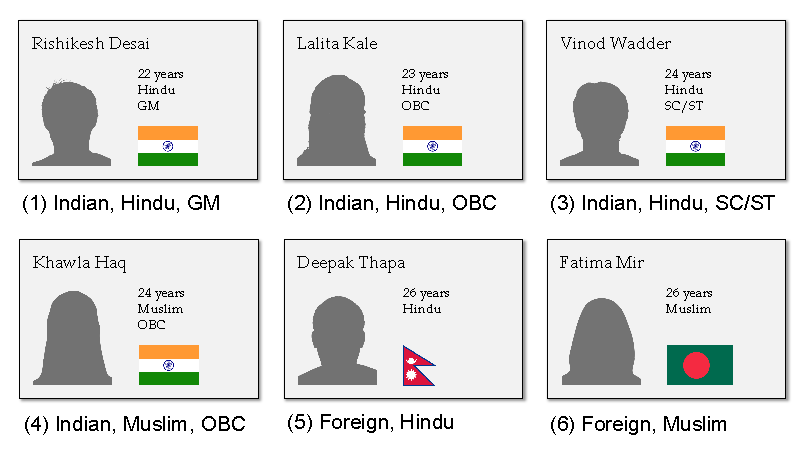
\includegraphics[scale=1]{../figures/figure-1}
\caption{
Schematic representations of social identity structures, ordered by social identity inclusiveness \protect\fullcite{dommelen_construing_2015}. Shaded regions represent the groups which a participant has to categorize as ``us'' to be assigned that structure. An Indian Hindu, for example, may consider only people who share their nationality, religion, and caste as ingroup members (intersection). Someone else may consider all their fellow Indians, whatever their religion or caste, as ingroup members (dominance). Another person may consider anyone who shares their nationality or religion as ingroup members (merger).
}
\label{fig:f1}
\end{figure}

Social psychologists have argued for the importance of considering two \cite{berry_immigration_1997, crisp_multiple_2007, dovidio_commonality_2009} or more \cite{roccas_social_2002} social categories for understanding intergroup relations. Broadly, these perspectives recognise that we are part of multiple overlapping groups; that we have a subjective sense of who is ``us'' and ``them'' that goes beyond the objective facts of group membership; and that identification across multiple categories affects our attitudes toward people with whom we share some, but not all, group memberships. However, these perspectives have lacked methods for measuring identification across multiple categories. Our research uses a novel method for studying subjective identity construals, as well as their antecedents (intergroup contact) and consequences (outgroup attitudes, intergroup threat, policy support).

Past research \shortcite{dommelen_construing_2015} studied whom individuals considered ``us'' and ``not us'', and observed substantial individual differences in how inclusive participants' social identities were. In this research, all participants belonged to the same groups. Group memberships, however, likely influences whom people consider ``us'' and ``not us''. For majority-group members, negotiating their ethnic and national identities means something different than for minority-group members \cite{dovidio_commonality_2009}. We expect that group differences are as great as, if not greater than, individual differences in social identity construals---especially if groups differ in status and power. Our research includes participants from diverse backgrounds to estimate these group differences.

Contact experiences could overcome group differences in social identity construals. Encountering diverse others could initiate a process of cognitive differentiation \cite{schmid_social_2011} whereby individuals become aware of complex interrelations between their group memberships, and thus start to question narrow identity construals. Further, positive intergroup interactions motivate people to include the outgroup of an interaction partner in their self-concept \cite{page_understanding_2010}. If contact motivates people to include partial outgroups in the self, it should encourage social identities that include the interaction partner's combination of group memberships. Together, these mechanisms suggest that contact could foster more inclusive identities.

Fostering more inclusive identities, in turn, could reduce intergroup bias. Dividing others into ``us'' and ``not us'' is a necessary and sufficient condition for ingroup favouritism \cite{tajfel_human_1981}. Considering more people as ``us'' should extend ingroup favouritism to a wider range of people, and thus reduce discrimination \cite{gaertner_common_2016}. Ingroup favouritism can turn into outgroup derogation when an outgroup threatens the ingroup \cite{brewer_psychology_1999}. Considering fewer people as ``not us'' should reduce the number of groups which are perceived to threaten the ingroup. Together, these mechanisms suggest that fostering inclusive identities could improve outgroup attitudes and reduce intergroup threat.

Beyond prejudice, researchers have debated whether fostering inclusive identities helps or hinders social change. Social change often requires advantaged and disadvantaged groups to strive for redistributive policies. On the one hand, fostering inclusive identities could break down the boundaries between the advantaged ingroup and the disadvantaged outgroup---turning injustice faced by ``them'' into ``our'' problem. This process could narrow the gap between advantaged-group members' support for the principle of equality and their opposition to its implementation \cite{dixon_intergroup_2007}. On the other hand, fostering more inclusive identities could distract disadvantaged-group members from differences in resources and power, and thus reduce their support for social change \cite{dovidio_darker_2012}. Together, these mechanisms suggest that more inclusive identities could increase support for social change among the advantaged, but decrease support among the disadvantaged.

\subsection{Caste, Religion, Nation in South India}

We tested these predictions among South Indian students, examining the cross-cutting categories of caste, religion, and nationality. Caste is a system of social relations that concentrates resources in the hands of dominant castes by restricting subordinate castes' occupations and land ownership, and by enforcing endogamy and segregation \cite{jodhka_caste_2012}. This system is underpinned by a tradition that ranks castes according to their supposed ritual purity, and condemns contact with less pure castes. Since Independence, the Indian State has sought to redress caste-based injustices by enforcing `reservations' of seats in state-run universities and state-sector jobs for disadvantaged groups. It recognises Dalits---members of castes affected by untouchability---as Scheduled Castes (SCs), Adivasi---India's indigenous peoples---as Scheduled Tribes (STs), and other disadvantaged groups---who occupy an intermediate position in the caste hierarchy---as Other Backward Classes (OBCs). Historically advantaged castes do not have access to reservations (GM: General Merit). Reservation policies, alongside ongoing discrimination, mean that caste identities remain important.

South India is religiously diverse. In Karnataka, where we conducted this research, 84\% of inhabitants are Hindus, while 13\% are Muslims. Muslims face both structural inequalities and communal violence. In 2002, for example, a pogrom killed over a thousand Muslims in Gujarat \cite{dhattiwala_political_2012}. In recent years, anti-Muslim violence has been increasing \cite{amnesty_india_2017}. Religion is intertwined with two currents of Indian nationalism \cite{menski_hindu_2009}. On the one hand, the secular foundations of the Indian State resulted from an inclusive nationalism that strives to include Indians of all religions. On the other hand, Hindu nationalism (Hindutva) is an ideology that equates being Indian with being Hindu, thus excluding Muslims from the national identity. Narendra Modi's BJP government espouses Hindutva, and enjoys broad support in the Indian population \cite{pew_three_2017}.

\section{Present research}

We examined how people construct their social identities from multiple group memberships---and whether intergroup contact can reduce prejudice, and increase support for social change, by fostering more inclusive identities. Our research used a novel method to study social identification across multiple categories in a sample of South Indians from various caste backgrounds.

First, we examined how participants' objective group memberships shaped their subjective construals of social identity.  We hypothesised that participants would exclude targets from religious and national outgroups---and that participants from advantaged castes would exclude targets from disadvantaged castes, and vice versa. We did not have a clear prediction for participants from intermediate caste groups. Second, we tested potential antecedents of more inclusive social identities. We hypothesised that positive contact and cross-group friendship would be associated with more, and negative contact with less, inclusive identities. As an alternative hypothesis, we tested whether ideological preferences for social dominance \cite{sidanius_social_1999} could have motivated individuals to exclude lower-status outgroups. Third, we examined potential consequences of participants' identity construals. We hypothesised that categorizing someone as ``us'' would be associated with more favourable attitudes and less social distance toward that person. More broadly, we expected more inclusive identities to be associated with less perceived intergroup threat. We also tested whether more inclusive identities would be associated with increased support for affirmative action among advantaged-group members, but decreased support among disadvantaged-group members.

We tested these predictions in a triple crossed-categorisation task (adapted from \citeNP{dommelen_construing_2015}). In this task, participants viewed identity cards, each representing a person with whom participants shared none, one, two, or all of three group memberships. Participants reported whether they considered each person as ``us'' or ``not us'', showing whom they included in, or excluded from, their ingroup. This task thus measured how participants combined multiple group memberships to construct their social identities. We tested to what extent participants' responses were associated with past contact experiences, ideological preferences, and various outcome measures.

\section{Method}

All materials, data, analysis scripts, and appendices are available online (\href{https://osf.io/ekb8z/?view_only=05b6a5c5cf5e43d9a7bba5e192f53f87}{https://osf.io/ ekb8z/?view\_only=05b6a5c5cf5e43d9a7bba5e192f53f87}). Here, we only report measures testing our hypotheses, omitting measures replicating earlier research or validating the categorization task (Appendix~E). Reanalysing existing data \cite{dommelen_construing_2015}, we determined that $\sim$100 respondents per group would allow reasonably precise estimates of model parameters.\footnote{Models estimated posterior probabilities with precision $\textit{SD} < 0.5$ on the log odds scale.}

\subsection{Participants}

We recruited 351 students at Karnatak University (Dharwad, India). Of these, we excluded 49 participants who did not belong to any of four caste groups ($n = 20$), failed to indicate their caste group ($n = 7$), or reported Islam as their own or their family's religion ($n = 27$).\footnote{We excluded Muslim participants as this subsample was too small for meaningful analyses.} This left 302 participants who reported Hinduism ($n = 286$), Jainism ($n = 8$), or Christianity ($n = 8$) as their or their family's religion, and General Caste ($n = 99$), Other Backward Class ($n = 127$), Scheduled Caste ($n = 54$), or Scheduled Tribe ($n = 22$) as their caste group. Table~\ref{tab:t1} summarises participants by gender, age, nationality, religion, and caste.

\begin{table}    
\caption[Participants by gender, age, nationality, religion, and caste]{Participants by gender, age, nationality, religion, and caste. Categories in \textit{italics} were excluded from the final sample. N/A marks missing responses.}
\centering
\figureversion{lining, tabular}
\small	
\begin{tabular}{llrr} \addlinespace \toprule
\multicolumn{2}{l}{Category} & $n$ & \% \\ \midrule \addlinespace 
Gender      & Woman      & 215 & 61 \\
            & Man & 121 & 34 \\
            & Other & 0 & 0 \\
            & N/A & 15 & 4 \\ \addlinespace \addlinespace
Age         & 18--20 & 1 & 0 \\
            & 21--23 & 254 & 72 \\
            & 24--26 &  77 & 22 \\
            & 27--29 &  10 &  3 \\
            & 30--32 &   1 &  0 \\
            & 33--35 &   0 &  0 \\
            & 36 or older & 1 & 0 \\ 
            & N/A & 7 & 2 \\ \addlinespace \addlinespace
Nationality & Indian & 339 & 97 \\
            & Other & 0 & 0 \\
            & N/A & 12 & 3 \\ \addlinespace \addlinespace
Religion    & Buddhism & 1 & 0 \\ 
            & Christianity & 11 & 3 \\ 
            & Hinduism & 297 & 85 \\ 
            & \textit{Islam} & \textit{27} & \textit{8} \\ 
            & Jainism & 8 & 2 \\ 
            & Other & 2 & 1 \\ 
            & N/A & 5 & 1 \\ \addlinespace \addlinespace
Caste       & General Caste & 104 & 30 \\ 
            & Other Backward Class & 143 & 41 \\ 
            & Scheduled Caste & 54 & 15 \\ 
            & Scheduled Tribe & 23 & 7 \\ 
            & \textit{Other / Not applicable} & \textit{20} & \textit{6} \\ 
            & \textit{N/A} & \textit{7} & \textit{2} \\ \addlinespace \midrule
Total       &   & 351 & 100 \\ \bottomrule
\end{tabular}
\label{tab:t1}
\end{table}

\subsection{Procedure}

Participants completed a triple crossed-categorization task, in which they viewed 24 identity cards. Each showed a fictitious person's name, age, religion, nationality, caste reservation, and a head-and-shoulders silhouette. Based on a pilot study, we manipulated the target's caste, religion, and nationality such that each target represented a person with whom participants shared none, one, two, or three group memberships (Figure~\ref{fig:f2}). We tested participants in classrooms of 24--71 students by presenting targets in a slide-based presentation. Each slide contained a male and a female target with participants focusing on the target corresponding to their gender. Slides also contained a number identifying each target, and the response scale(s) corresponding to the question(s) participants answered at the time. 

\begin{figure}
\centering
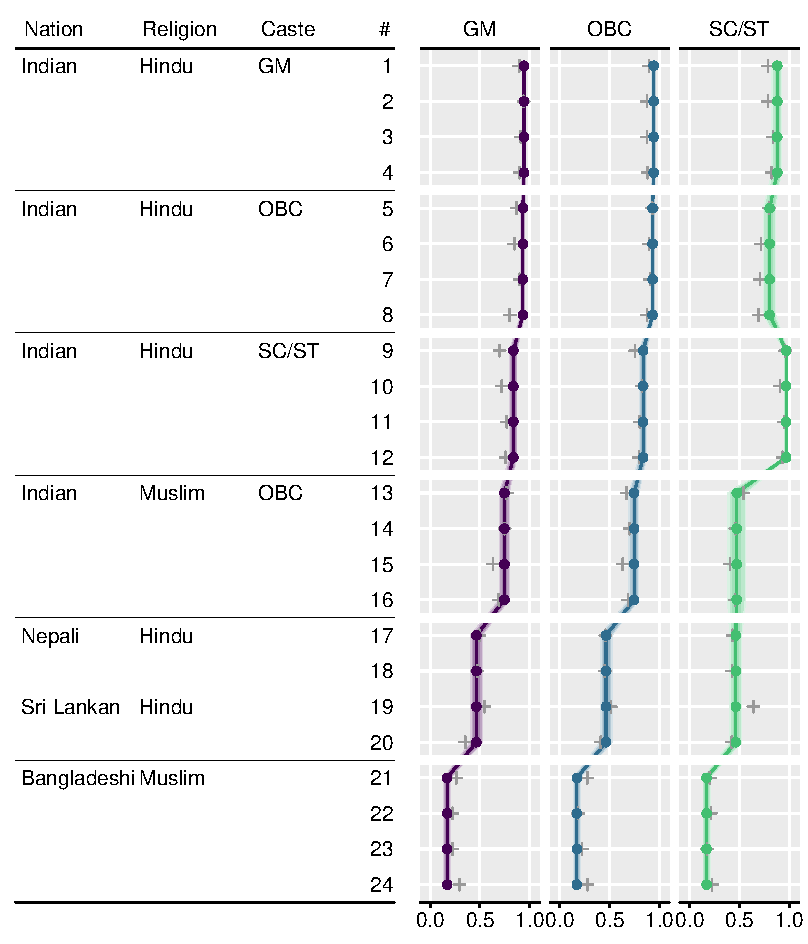
\includegraphics[scale=1]{../figures/figure-2}
\caption{Examples of targets used in the triple crossed-categorization task. Based on ratings in a pilot study ($N = 26$), we selected the four most prototypical targets (out of fifty initial targets) for each of six plausible combinations of caste, religion, and nationality (for details, see Appendix~A). Each target showed a person's caste (GM = General Merit, OBC = Other Backward Class, SC/ST = Scheduled Caste/Scheduled Tribe), religion (Hindu, Muslim), and nationality (Indian, Nepali, Sri Lankan, Bangladeshi). Each target also showed the person's first and last name, age (21--26 years), and a silhouette corresponding to the person's gender (adapted from \protect\citeNP{ma_chicago_2015}). Each target's age and silhouette, as well as the order in which the targets were presented, varied across sessions.}
\label{fig:f2}
\end{figure}

In each session, participants first familiarised themselves with each target (for 7s) in an automated slideshow. Participants viewed targets (in the same order) for a second time, noting for each target whether they felt that this person was one of their own group (1 = ``us''), or not one of their own group (0 = ``not us''). Participants viewed targets for a third time, rating how comfortable or uncomfortable they would feel to share a room with this person (social distance; $1 = \textit{very uncomfortable}$, $7 = \textit{very comfortable}$), and how they felt toward this person (feeling thermometer; $0 = \textit{cold}$, $\textit{100 = warm}$). Participants then completed a questionnaire containing the measures described below. 

\subsection{Measures}

We measured intergroup contact as: how often, from $1 = \textit{never}$ to $5 = \textit{very often}$, participants meet outgroup members in their everyday life (contact quantity), and how often, on average, they have positive/good contact and negative/bad contact with outgroup members \cite{barlow_contact_2012}. We preceded these items with examples of positive and negative contact experiences. We measured cross-group friendship with two items \cite{turner_reducing_2007}: ``How many close friends do you have who are [outgroup members]?'' ($1 = \textit{none}$, $5 = \textit{more than ten}$), and ``How often do you spend time with [outgroup] friends?'' ($1 = \textit{never}$ to $5 = \textit{very often}$; $.47\leq\textit{rs}\leq.58$). Participants reported contact with four groups: Dalits, people from other backward classes, people from general castes, and Muslims.

We measured social dominance orientation as how much, between $1 = \textit{strongly oppose}$ and $7 = \textit{strongly favour}$, participants endorsed eight statements about social hierarchies \cite{ho_nature_2015}. Four items measured support for group-based dominance (SDO-Dominance), e.g., ``some groups of people are simply inferior to other groups''. Four items measured opposition to egalitarian ideologies (SDO-Egalitarianism), e.g., ``it is unjust to try to make groups equal''.\footnote{Replicating \citeauthor{ho_nature_2015}’s \citeyear{ho_nature_2015} findings, we found a four-factor model (with two method factors) to represent the data better than the one-factor ($\Delta\chi^2 = 155.14$, $p < .001$) or two-factor ($\Delta\chi^2 = 138.67$, $p < .001$) alternatives. Accounting for this structure, we used latent factor scores for SDO-Dominance and SDO-Egalitarianism in our analyses.}

We measured realistic threat---from Muslims and Dalits---with three items per outgroup \cite{schmid_reducing_2014}, e.g., ``the more power [Muslims/Dalits] gain in this country, the more difficult it is for [Hindus/people from my caste group]'' ($1 = \textit{strongly disagree}$, $5 = \textit{strongly agree}$; $\alpha_\textit{Muslims} = .71$, $\alpha_\textit{Dalits} = .79$). Two items measured symbolic threat, e.g., ``[Muslims/Dalits] threaten [Hindus'/my caste group's] way of life'' ($1 = \textit{strongly disagree}$, $5 = \textit{strongly agree}$; $r_\textit{Muslims} = .44$, $r_\textit{Dalits} = .48$).

We measured perceived (dis-)advantage as how easy or hard participants thought it was, on average, for people from various groups to succeed in India today ($1 = \textit{very hard}$, $7 = \textit{very easy}$). Participants rated seven groups: People from your own background, Scheduled Caste, Scheduled Tribe, Other Backward Class, General Caste, Hindus, and Muslims.

Five items measured policy support. Participants read that ``currently, 22.5\% of seats in central-government funded universities are reserved for Scheduled Caste and Scheduled Tribe students'', and that ``an additional 27.5\% of seats in central-government funded universities are reserved for students from Other Backward Classes''. Participants indicated to what extent they opposed or supported reservation in higher education for students from each group ($1 = \textit{strongly oppose}$, $5 = \textit{strongly support}$), and whether they thought that reservation in higher education for students from that group should increase, decrease, or remain unchanged ($1 = \textit{decrease a lot}$, $5 = \textit{increase a lot}$; $r_\textit{SC/ST} = .67$, $r_\textit{OBC} = .67$). Participants then read that ``no seats in central-government funded universities are reserved for Muslim students nationally, though some states have introduced quotas for Muslim students''. Participants indicated to what extent they opposed or supported reservation for Muslim students.

\section{Results}

We used the following analysis strategy: First, we estimated group differences in whom participants categorized as ``us'' and ``not us''. Second, we examined to what extent intergroup contact and ideological orientations explained individual differences in participants' categorizations. Third, we tested whether participants' categorizations were associated with their attitudes and beliefs.

\subsection{Group differences}

We compared \emph{how likely} participants were to categorize \emph{which} target as ``us'' versus ``not us''---and how that probability varied across targets' and participants' group memberships.\footnote{In Appendix~B, we report analyses using \citeauthor{dommelen_construing_2015}'s \citeyear{dommelen_construing_2015} operationalisation who analysed which and how many targets participants included as distinct questions. }

We estimated a series of Bayesian multilevel models in RStan \cite{rstan_package} with participants' target categorizations ($1 = \text{``us''}$, $0 = \text{``not us''}$) as outcome variable. Models derived the likelihood of the observed proportions of ``us'' categorizations from the Bernoulli likelihood with a logit link function. Models assigned weakly informative prior distributions to all fixed parameters \cite{gelman_prior_2017}.\footnote{Models assigned the following priors: $\beta \sim \text{Student}(2.5, 0, 1)$ for fixed effects, and $\sigma \sim \text{Cauchy}(0, 1)$ for standard deviations of varying effects.} Models used the non-centred parameterisation for all varying effects \cite{betancourt_hamilton_2015}. We compared models using stratified 10-fold cross-validation to estimate each model's out-of-sample predictive accuracy \shortcite{vehtari_practical_2017}. We selected more complex over simpler models when the difference in predictive accuracy was at least twice its standard error.

Models~0 to 3 estimated the probabilities of ``us'' categorizations as varying between participants but fixed across target categories (M0), as varying across participants and target categories (M1), and tested whether SC/ST participants' categorizations of Indian targets differed from GM and OBC participants' (M2) and whether OBC participants’ categorizations differed from GM participants' (M3). Models~1 and 2, but not Model~3, made more accurate predictions than less complex models (Table~\ref{tab:t2}). This suggests that the targets' group memberships shaped participants' categorizations, and that GM and OBC participants' categorizations resembled each other but differed from SC/ST participants'. Below, we report median point estimates, with 97\% highest posterior density intervals \cite{coda_package}, from the model's posterior distribution.

\begin{table}
\caption{
Comparison of models estimating the probability of participants categorising targets as ``us'' versus ``not us''. $\textit{ELPD}$ is the expected log predictive density, with higher numbers indicating that a model is expected to make more accurate out-of-sample predictions \protect\fullcite{vehtari_practical_2017}. $\Delta\textit{ELPD}$ is the difference in $\textit{ELPD}$ between the current and previous model, with positive values indicating that the current model is expected to make more accurate out-of-sample predictions. We selected a more complex model over a simpler model when $\frac{\Delta\textit{ELPD}}{\textit{SE}} \geq 2$. $w$ are stacking weights based on the models' expected log predictive densities \protect\cite{yao_using_2018}.
}
\centering
\figureversion{lining, tabular}
\small
\begin{tabularx}{\linewidth}{r@{~}rXrrrrrr} \toprule
\# &  & Description & $\textit{ELPD}$ & $\textit{SE}$ & $\Delta\textit{ELPD}$ & $\textit{SE}$ & $\frac{\Delta\textit{ELPD}}{\textit{SE}}$ & $w$ \\ \midrule 
0 &      & Intercept (Participant) & -4703.5 & 23.7 &     - &    - &    - & .00 \\ 
1 & vs 0 & Intercept (Category)    & -3853.5 & 41.6 & 850.1 & 37.4 & 22.7 & .00 \\
2 & vs 1 & Group differences (SC/ST)       & -3791.3 & 42.0 &  62.1 & 11.1 &  5.6 & .00 \\
3 & vs 2 & Group differences (OBC)         & -3792.1 & 42.2 &  -0.8 &  3.6 & -0.2 & .07 \\ \midrule
4 & vs 2 & Intergroup contact (4) & -3743.4 & 42.8 &  47.9 &  8.8 &  5.4 & .00 \\
5 & vs 4 & Intergroup contact (2) & -3736.7 & 42.6 &   6.7 &  1.8 &  3.8 & .92 \\
6 & vs 5 & Intergroup contact (2) & -3747.8 & 42.7 & -11.1 &  3.2 & -3.5 & .00 \\
7 & vs 2 & Social dominance orientation & -3791.0 & 42.1 &   0.4 &  3.3 &  0.1 & .00 \\
\bottomrule
\end{tabularx}
\label{tab:t2}
\end{table}

Figure~\ref{fig:f3} shows the estimated probabilities of General Merit (GM), Other Backward Class (OBC), and Scheduled Caste/Scheduled Tribe (SC/ST) participants categorizing a target as ``us''. Participants tended to define their ingroup in terms of nationality, though about half of the responses indicated more inclusive identities. Few participants considered Bangladeshi Muslims part of their ingroup, \pest{M2}{.17}{.14}{.21}. Roughly half of the participants included Sri Lankan and Nepali Hindus in their ingroup, \pest{M2}{.46}{.41}{.52}. Participants were thus more likely to include foreign targets when they were Hindu, \pdif{M2}{.29}{.25}{.34}. Still, GM/OBC and SC/ST participants were, respectively, $1.95$, $[1.73, 2.18]$ and $1.90$, $[1.71, 2.14]$ times more likely to categorize Indian, Hindu targets as ``us'' compared to foreign, Hindu targets.

\begin{figure}
\centering
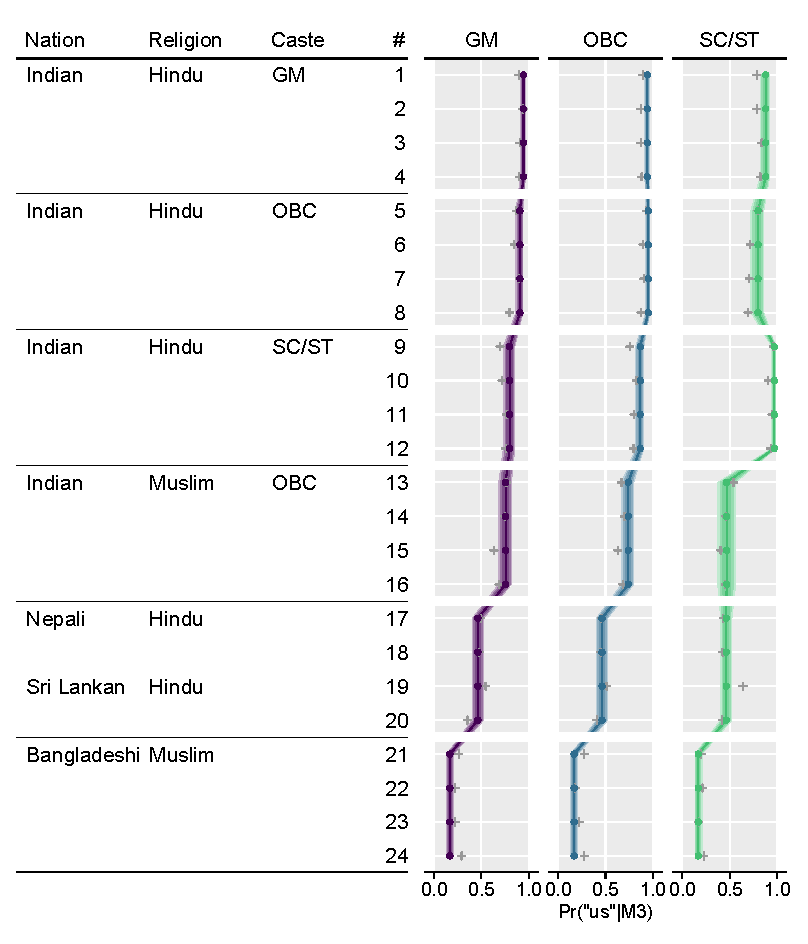
\includegraphics[scale=1]{../figures/figure-3}
\caption{
Estimated probability of participants categorizing a target as ``us'' versus ``not us'' by targets' nationality, religion, and caste (vertical), and participants' caste membership (horizontal). Dots (•) indicate the most plausible \emph{estimate} for a given target's probability of being included in participants' ingroup (in Model~2, Table~\ref{tab:t2}), while the shaded ribbons encompass the 67\% (darkest shade), 89\%, and 97\% (lightest shade) most plausible estimates of that probability. Pluses (+) indicate the \emph{observed} proportion of participants who included a given target in their ingroup. Comparing predicted and observed proportion shows that the model represents the data reasonably well. GM = General Merit, OBC = Other Backward Class, SC/ST = Scheduled Caste/Scheduled Tribe.
}
\label{fig:f3}
\end{figure} 

As expected, participants' caste membership shaped how they categorized Indians of different castes and religions. Most GM and OBC participants included \emph{Hindu, GM} and \emph{Hindu, OBC} targets in their ingroup, \pest{M2}{.94}{.92}{.96} and \pest{M2}{.93}{.91}{.95}. Fewer GM and OBC participants categorized \emph{Hindu, SC/ST} targets as ``us'', \pest{M2}{.84}{.80}{.87}. They were least likely to categorize \emph{Muslim, OBC} targets as ``us'', \pest{M2}{.75}{.70}{.80}. Dalit/Adivasi (SC/ST) participants' responses differed from GM and OBC participants'. Almost all SC/ST participants included \emph{Hindu, SC/ST} targets in their ingroup, \pest{M2}{.97}{.95}{.99}. Fewer SC/ST participants included \emph{Hindu, GM} and \emph{Hindu, OBC} in their ingroup, \pest{M2}{.88}{.83}{.92} and  and \pest{M2}{.80}{.73}{.86}. SC/ST participants were less likely than others to include \emph{Muslim, OBC} targets as ``us'', \pest{M2}{.47}{.38}{.57}. These findings showed that participants from advantaged backgrounds tended to exclude targets from disadvantaged backgrounds (and vice versa), while all participants tended to exclude targets from the Muslim minority.

\subsection{Individual differences}

We examined to what extent individual differences in past experiences and ideological orientations explain why some participants excluded targets from caste and religious outgroups---and why others did not.

Models~4 to 6 tested whether intergroup contact was associated with how participants categorized Indian targets of caste or religious outgroups. Model~4 extended Model~2 by including contact quantity, positive contact, negative contact, and outgroup friendship as predictors of participants' categorizations. Model~4 made more accurate predictions than Model~2. Negative contact ($e^\beta = 0.81$, $[0.72, 0.90]$) and outgroup friendship ($e^\beta = 1.50$, $[1.28, 1.72]$) were associated with participants' categorizations, but neither positive contact ($e^\beta = 1.01$, $[0.87, 1.16]$) nor contact quantity ($e^\beta = 0.99$, $[0.86, 1.15]$) were. Model~5 included only negative contact and outgroup friendship, and made more accurate predictions than Model~4. Model~6 estimated the relationships between contact and categorizations as varying across the four combinations of target caste and religion. Model~6 made less accurate predictions than Model~5.

Figure~\ref{fig:f4} shows the estimated probabilities of participants categorizing targets as ``us'' as a function of contact experiences. Across targets and participants, the odds of categorizing an outgroup target as ``us'' were $e^\beta = 1.50$, $[1.32, 1.69]$ times higher for each additional standard deviation of outgroup friendship. These odds were $e^\beta = 0.81$, $[0.72, 0.90]$ times lower for each standard deviation of negative contact. This means, for example, that GM/OBC participants who reported ``never'' having any negative contact with Muslims were more likely to categorize Indian Muslims as ``us'' than participants who reported ``sometimes'' having negative contact, \pdif{M5}{.05}{.09}{.03}. GM/OBC participants who reported no friendships with Muslims were a lot less likely to include Indian Muslims in their ingroup than participants who had 2--5 Muslim friends with whom they ``sometimes'' spent time, \pdif{M5}{.18}{.12}{.24}. Contact experiences were thus associated with whom participants categorized as ``us'' and ``not us''.

\begin{figure}
\centering
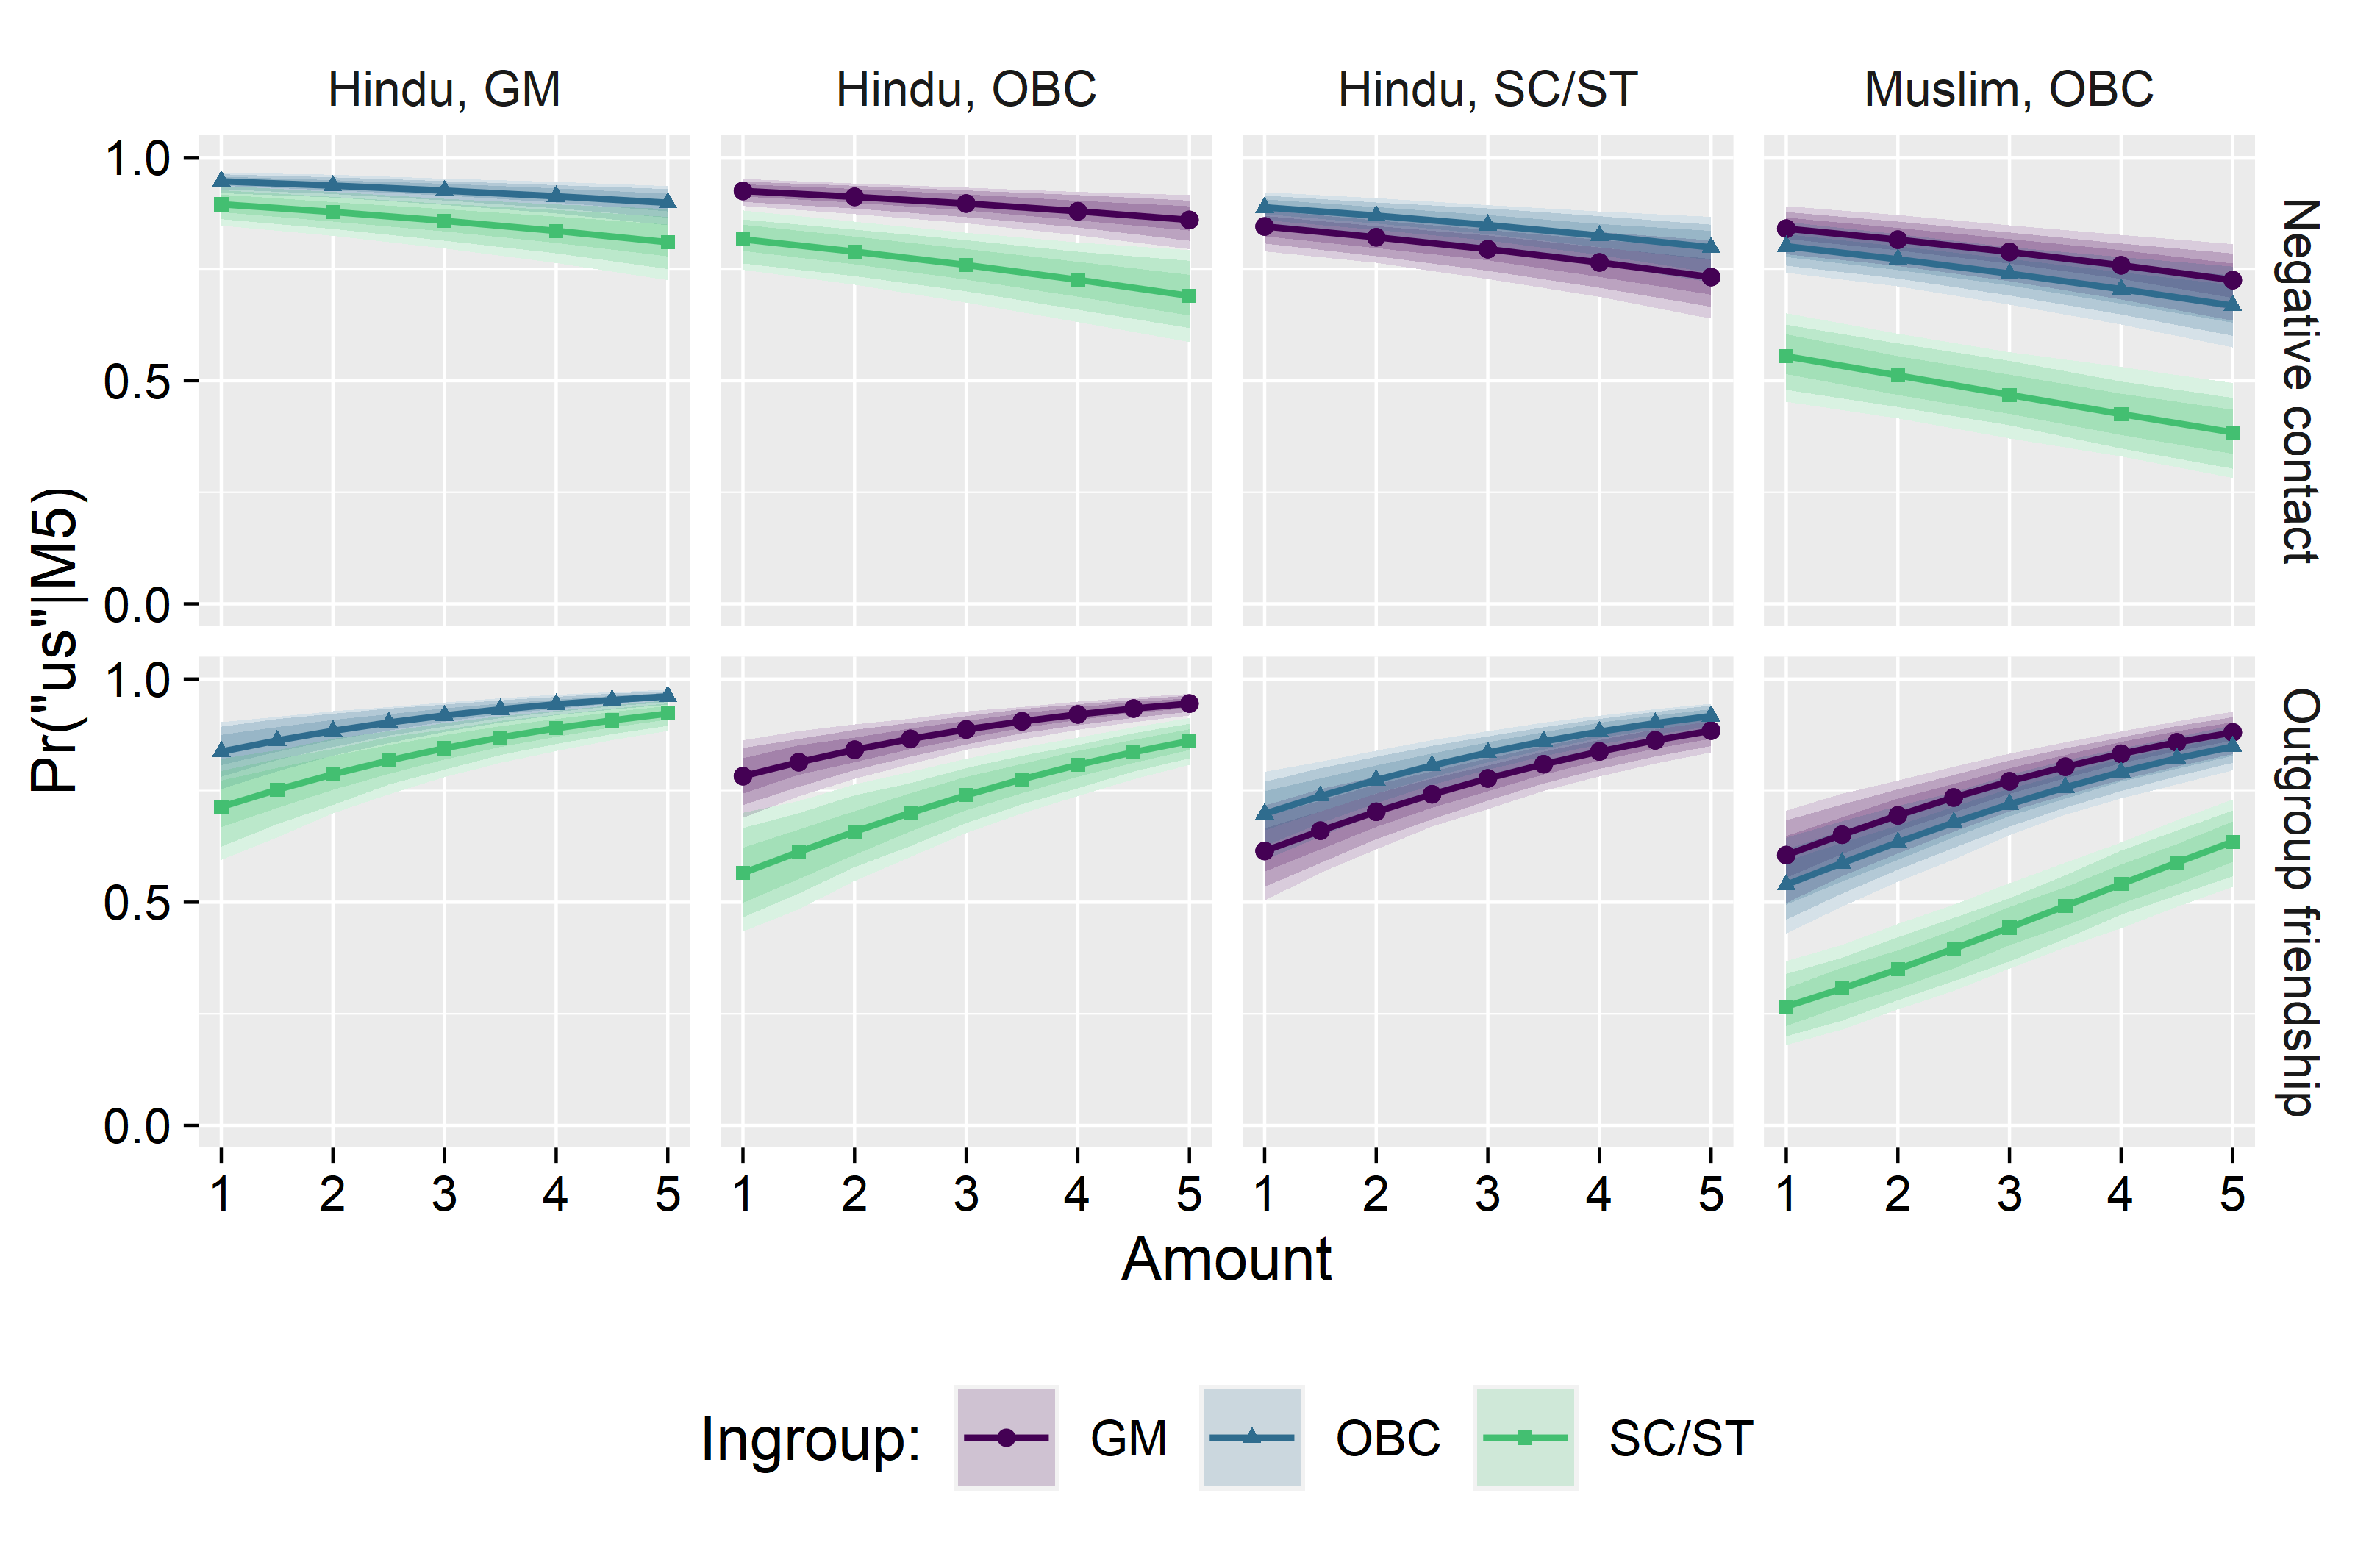
\includegraphics[scale=1]{../figures/figure-4}
\caption{Estimated probability of participants categorising a target as ``us'' versus ``not us'' as a function of the targets' group memberships (horizontal), the participants' group memberships (colour), and the reported amount of negative contact and outgroup friendship with the relevant groups (in Model~5, Table~\ref{tab:t2}). GM = General Merit, OBC = Other Backward Class, SC/ST = Scheduled Caste/Scheduled Tribe.}
\label{fig:f4}
\end{figure}

Models~7 tested whether social dominance orientation was associated with participants' categorizations of targets from lower status outgroups. Model~7 found little evidence for associations between participants' categorizations and their SDO-Dominance scores ($e^\beta = 0.87$, $[0.69, 1.06]$) or SDO-Egalitarianism scores ($e^\beta = 0.98$, $[0.78, 1.21]$). Together, these findings show that group and individual differences explained whom participants included in their ingroup. As expected, past experiences with outgroup members explained why some participants included targets of (objective) caste or religions outgroups in their (subjective) ingroup, when others did not. In contrast, ideological orientations did not motivate participants to exclude lower-status groups.

\subsection{Consequences}

We analysed how participants' categorizations related to their warmth and social distance ratings for each target in the categorization task, to intergroup threat, and to their perceived (dis-)advantage and policy support.

We estimated multivariate models with participants' target-wise social distance and feeling thermometer ratings as outcome variables (Table~\ref{tab:t3}). Models~0 to 3 estimated ratings (on either outcome) as varying between participants but fixed across targets (M0), as varying across participants and targets (M1), and tested whether SC/ST participants' responses differed from GM and OBC participants' (M2), and whether OBC participants' responses differed from GM participants (M3). Models~1 to 3 improved upon the predictions of simpler models, showing that participants' ratings depended on targets' and participants' group memberships.

\begin{table}
\caption{Comparison of models estimating participants' social distance (SD) and feeling thermometer (FT) ratings for each target as a function of group differences and target categorizations. As in Table~\ref{tab:t2}, we selected a more complex model over a simpler model when $\frac{\Delta\textit{ELPD}}{\textit{SE}} \geq 2$. $R^2$ is a Bayesian analogue to $R^2$ in maximum likelihood estimation \protect\fullcite{gelman_rsquared_2017}.}
\centering
\figureversion{lining, tabular}
\small	
\begin{tabularx}{\linewidth}{r@{~}rXrrrrrrrr} \toprule
\# &  & Description & $R^2_\text{SD}$ & $R^2_\text{FT}$ & $\textit{ELPD}$ & $\textit{SE}$ & $\Delta\textit{ELPD}$ & $\textit{SE}$ & $\frac{\Delta\textit{ELPD}}{\textit{SE}}$ & $w$ \\ \midrule 
0 &      & Participant & .23 & .26 & -16964 & 71.0 & - & - & - & .12 \\
1 & vs 0 & Category & .38 & .42 & -16338 & 79.6 & 626.8 & 40.2 & 15.6 & .02 \\
2 & vs 1 & SC/ST    & .38 & .43 & -16317 & 79.6 &  20.1 &  9.8 &  2.1 & .00 \\
3 & vs 2 & OBC      & .39 & .43 & -16293 & 80.5 &  24.2 &  9.7 &  2.5 & .00 \\ \midrule
4 & vs 3 & Categorization    & .42 & .47 & -16028 & 83.5 & 264.8 & 24.5 & 10.8 & .19 \\
5 & vs 4 & \ldots~(Category) & .42 & .47 & -16007 & 83.6 &  21.1 &  8.7 &  2.4 & .67 \\
6 & vs 5 & \ldots~(Ingroup)  & .42 & .47 & -16025 & 84.3 & -17.4 &  5.9 & -3.0 & .00 \\
\bottomrule    
\end{tabularx}
\label{tab:t3}
\end{table}

Models~4 to 6 tested whether participants who categorized a target as ``us'' rated that target more favourably than participants categorizing the same target as ``not us''. Models estimated this difference as constant across targets and participants (M4), as varying across target categories (M5), and tested whether this difference depended on participants' caste memberships (M6). Models 4 and 5, but not Model 6, made better predictions than less complex models, showing that how favourably participants felt toward a target depended on whether they had categorized that target as ``us'' or ``not us'', and that the size of this difference depended on the targets'---but not the participants'---group memberships.

Figures~\ref{fig:f5} and \ref{fig:f6} show, respectively, the estimated social distance and feeling thermometer ratings as a function of target categorizations and participants' caste memberships. For all categories, participants felt more comfortable sharing a room with targets that they categorized as ``us'' than with targets they categorized as ``not us''.  This difference was smallest for \emph{Indian, Hindu, GM} targets ($\beta = 0.55$, $[0.19, 0.90]$; $d = 0.24$, $[0.08, 0.39]$) and greatest for \emph{foreign, Muslim} targets ($\beta = 1.46$, $[1.21, 1.70]$; $d = 0.63$, $[0.52, 0.73]$). We found a similar pattern for feeling thermometer ratings. The difference was smallest for \emph{Indian, Hindu, OBC} targets ($\beta = 6.5$, $[2.1, 11.0]$, $d = 0.20$, $[0.06, 0.33]$) and greatest for \emph{foreign, Hindu} targets ($\beta = 21.8$, $[18.6, 25.0]$, $d = 0.66$, $[0.56, 0.76]$). Feeling thermometer and social distance ratings were highly correlated ($r = .58$, $[.56, .60]$). Categorizing a target as ``us'' was thus associated with more warmth and less social distance toward that target.

\begin{figure}
\centering
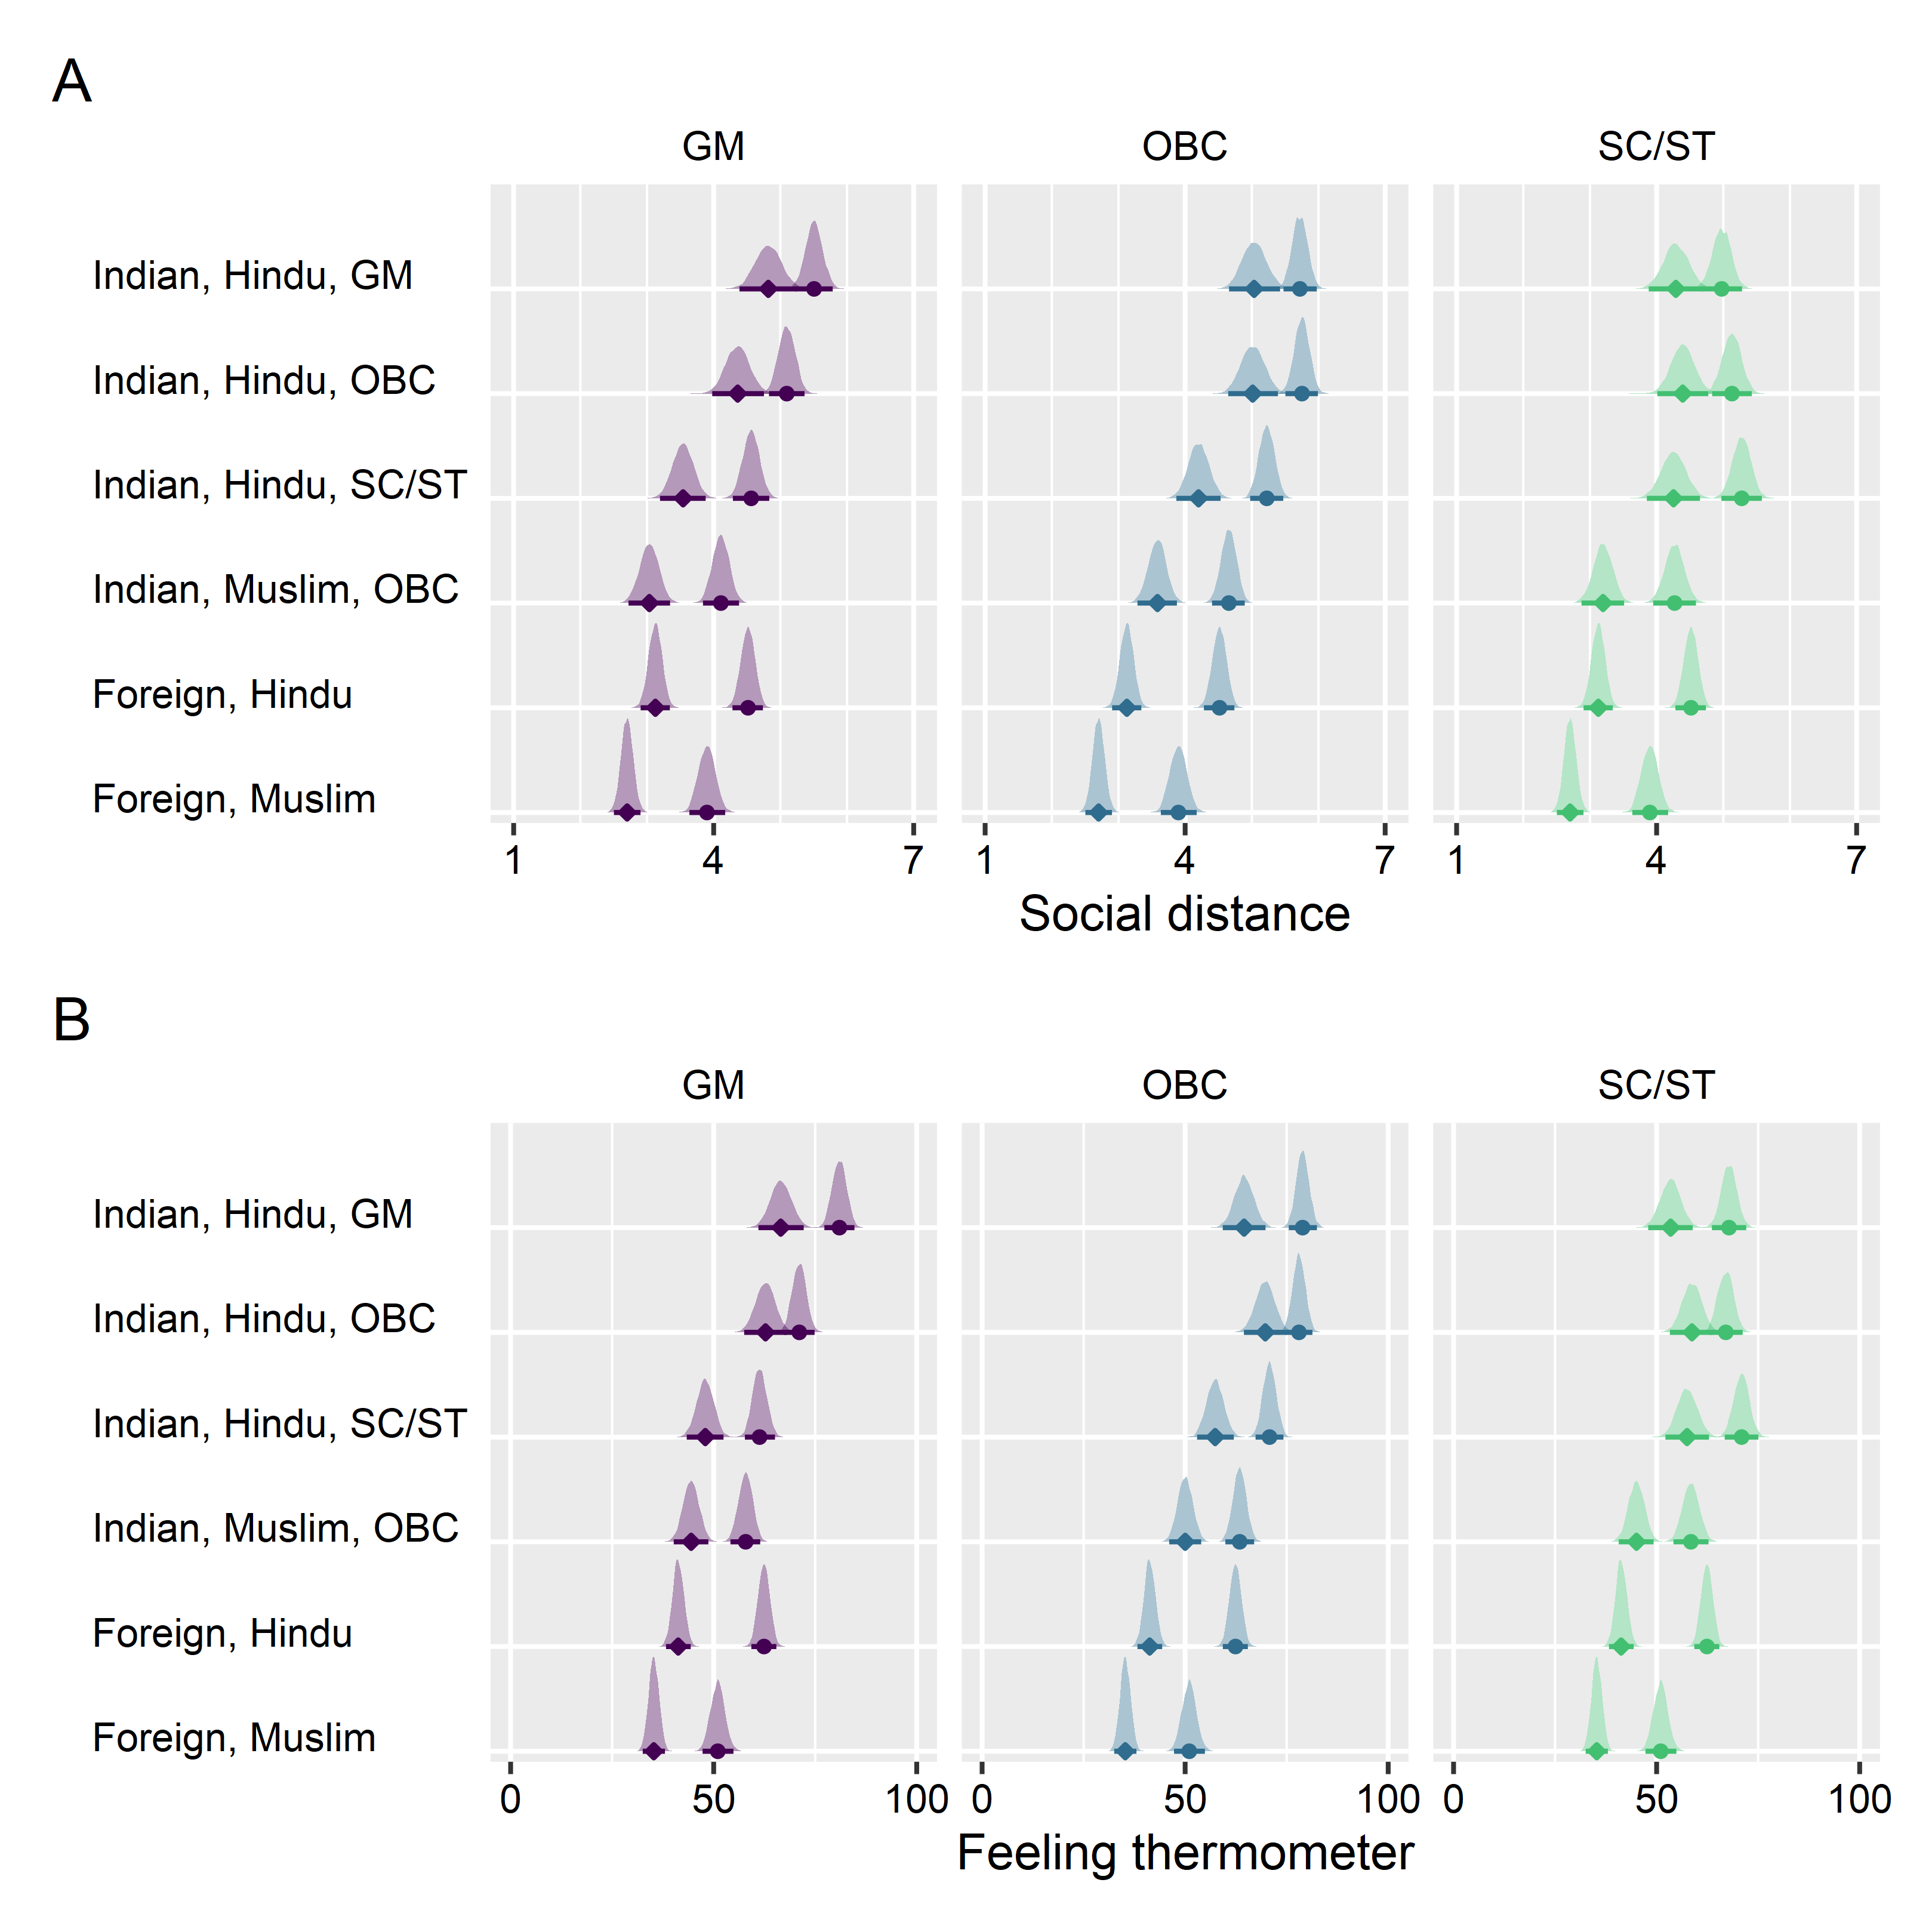
\includegraphics[scale=1]{../figures/figure-5}
\caption{
Posterior probabilities of social distance ratings as a function of target categorizations (in Model~5, Table~\ref{tab:t3}). Points are the estimated mean ratings for targets categorized as ``us''; triangles are the estimated mean ratings for targets categorized as ``not us''. GM = General Merit, OBC = Other Backward Class, SC/ST = Scheduled Caste/Scheduled Tribe.
}
\label{fig:f5}
\end{figure}

\begin{figure}
\centering
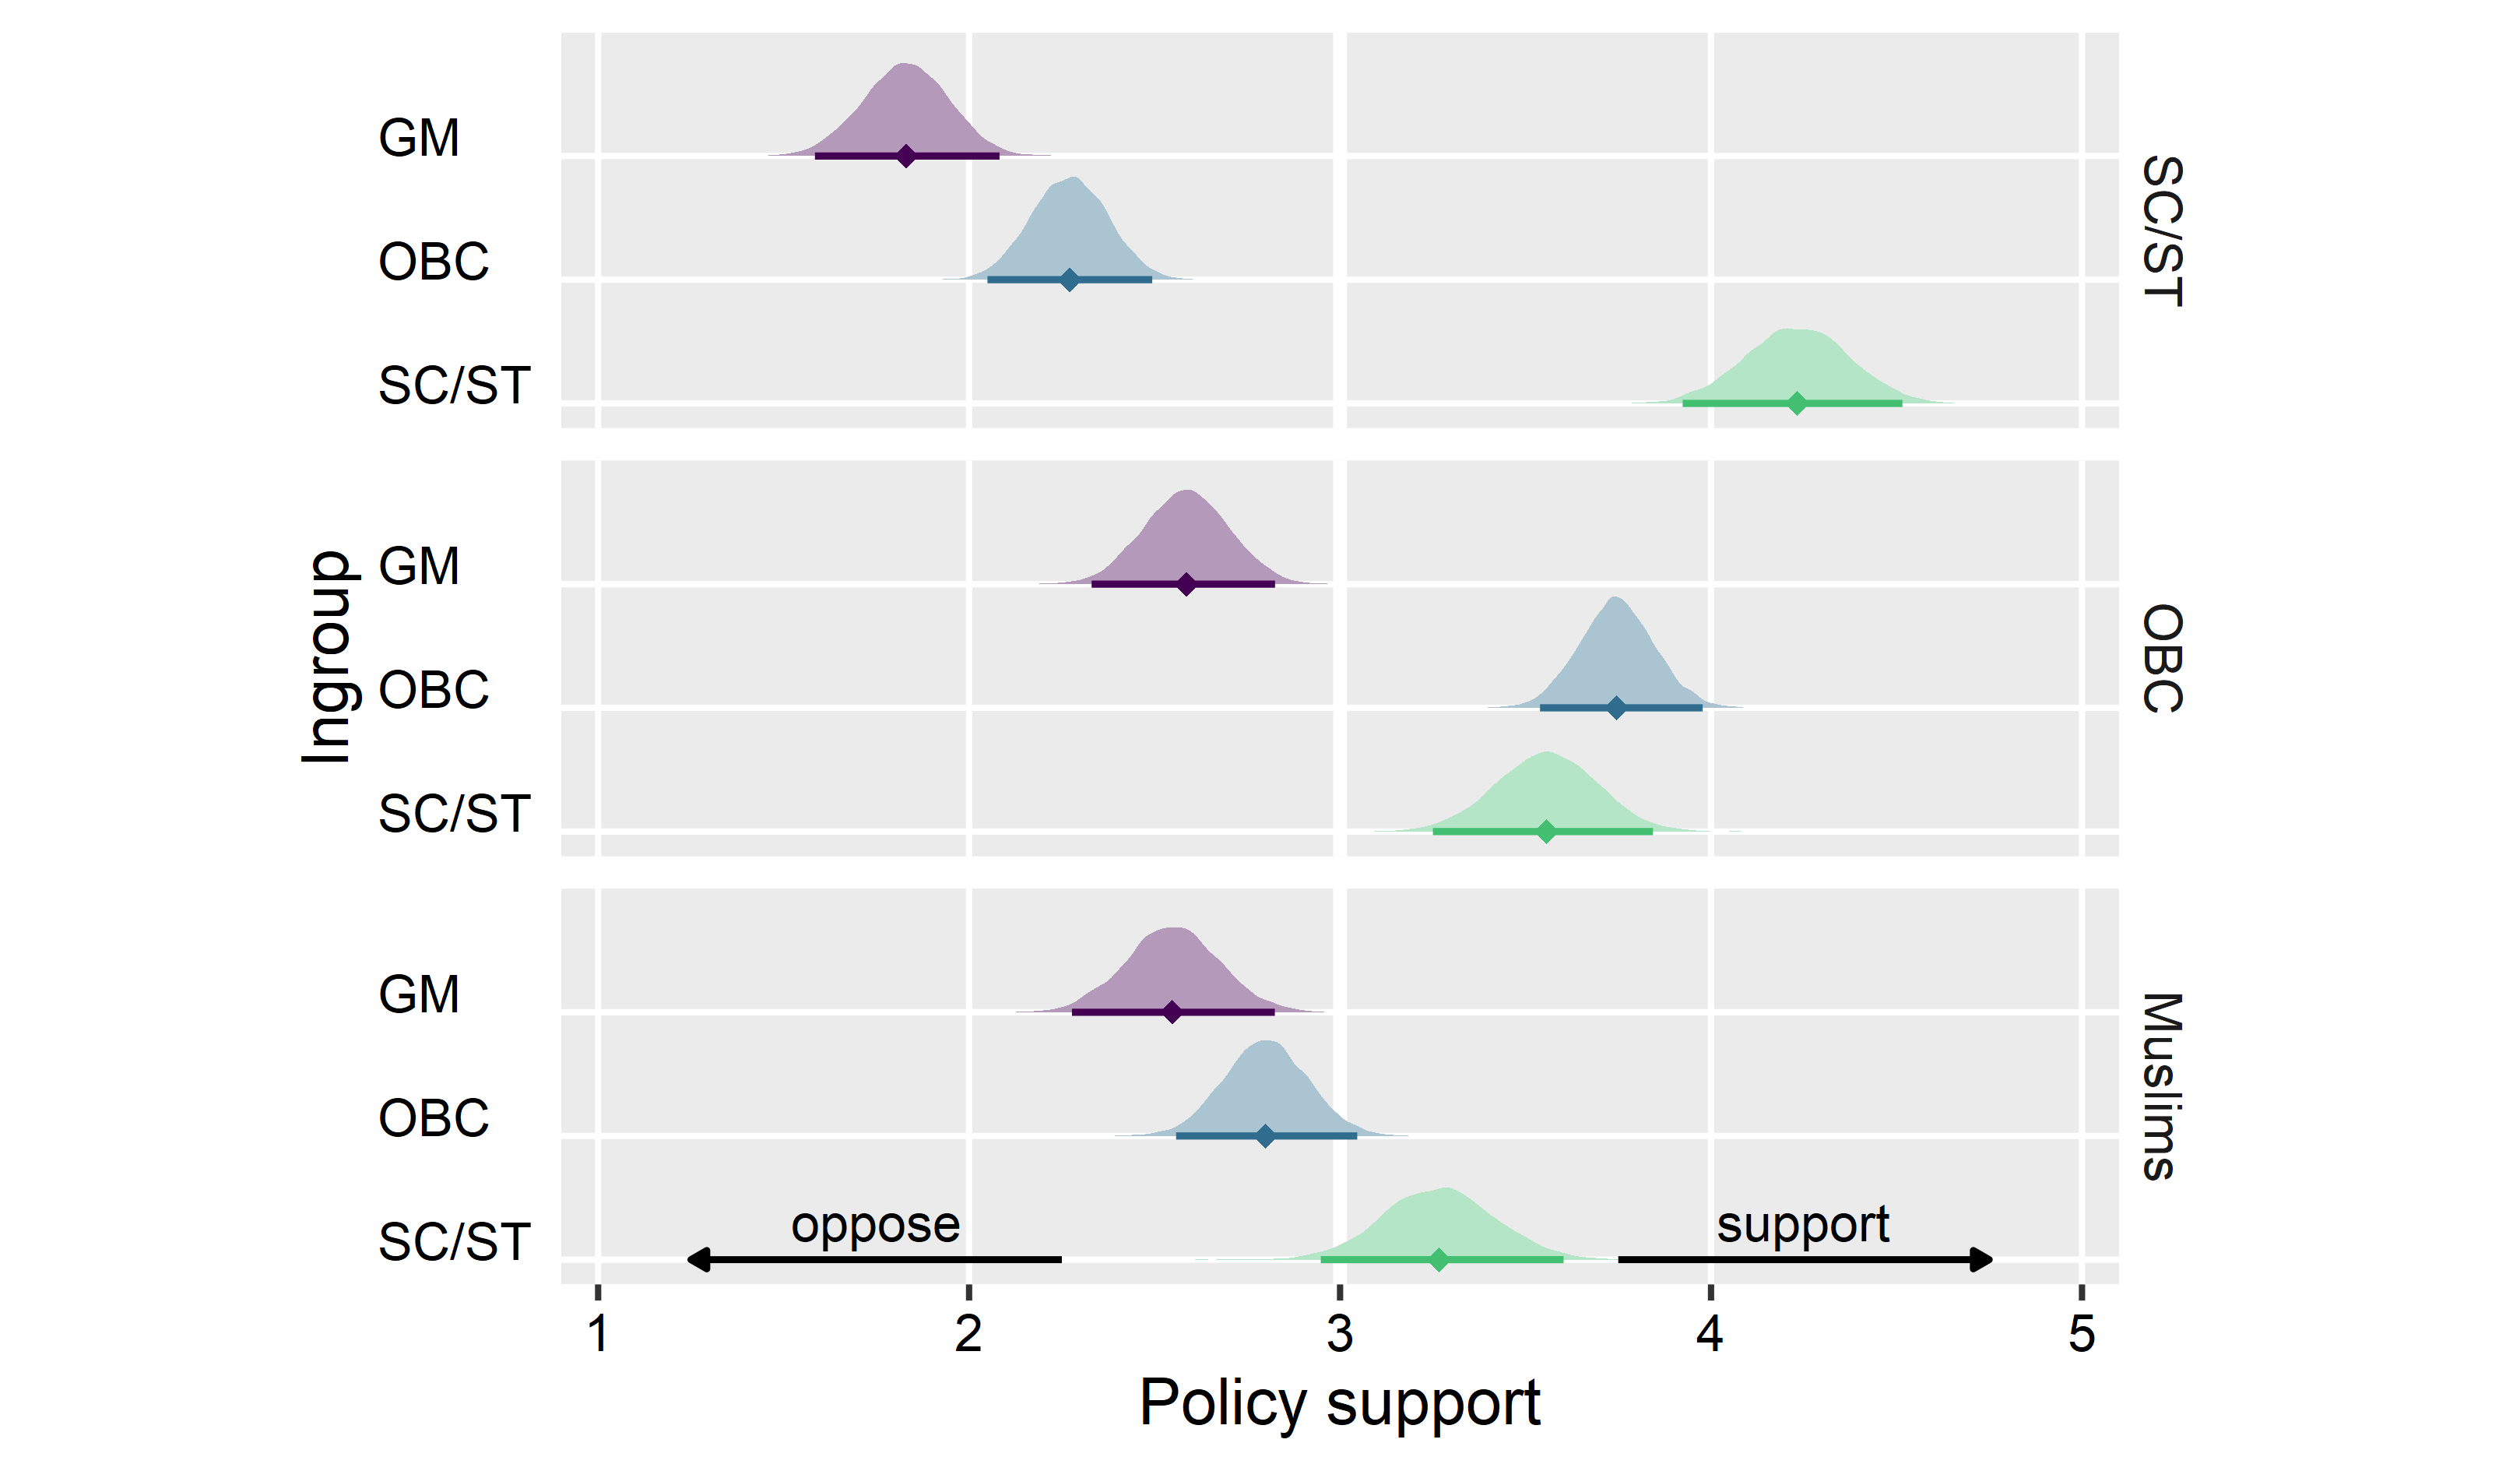
\includegraphics[scale=1]{../figures/figure-6}
\caption{
Posterior probabilities of feeling thermometer ratings as a function of target categorizations (in Model~5, Table~\ref{tab:t3}). Points are the estimated mean ratings for targets categorized as ``us''; triangles are the estimated mean ratings for targets categorized as ``not us''. GM = General Merit, OBC = Other Backward Class, SC/ST = Scheduled Caste/Scheduled Tribe.
}
\label{fig:f6}
\end{figure}

Next, we tested whether participants' perceptions of realistic and symbolic threat depended on how inclusive their identity construals were. Results from a series of multilevel models showed that participants reported more realistic ($M = 3.62$, $[3.49, 3.75]$) than symbolic ($M = 3.21$, $[3.09, 3.33]$) threat from (same-religion) Dalits, but more symbolic ($M = 3.47$, $[3.34, 3.61]$) than realistic ($M = 3.23$, $[3.06, 3.38]$) threat from (different-religion) Muslims. Contrary to predictions, we did not find that participants felt less threatened by Muslims and Dalits if they categorized more targets from these outgroups as ``us''. For details, see Appendix~C.

Finally, we estimated group differences in perceived (dis-)advantage and policy support. Figures~\ref{fig:f7} and \ref{fig:f8} show the estimated group differences in both outcomes. Contradicting prevailing social inequalities, GM and OBC participants rated their own groups' lives as substantially harder than SC/ST members' lives. Policy support strongly aligned with participants' caste interests. SC/ST participants supported reservations for both SC/ST and OBC students, while OBC participants only supported reservations for their own group. Contrary to predictions, we did not find more inclusive identities to be associated with either perceived (dis-)advantage or policy support. Contrary to past research \cite{dixon_beyond_2012}, intergroup contact was similarly unrelated to these outcomes. For details, see Appendix~D.

\begin{figure}
\centering
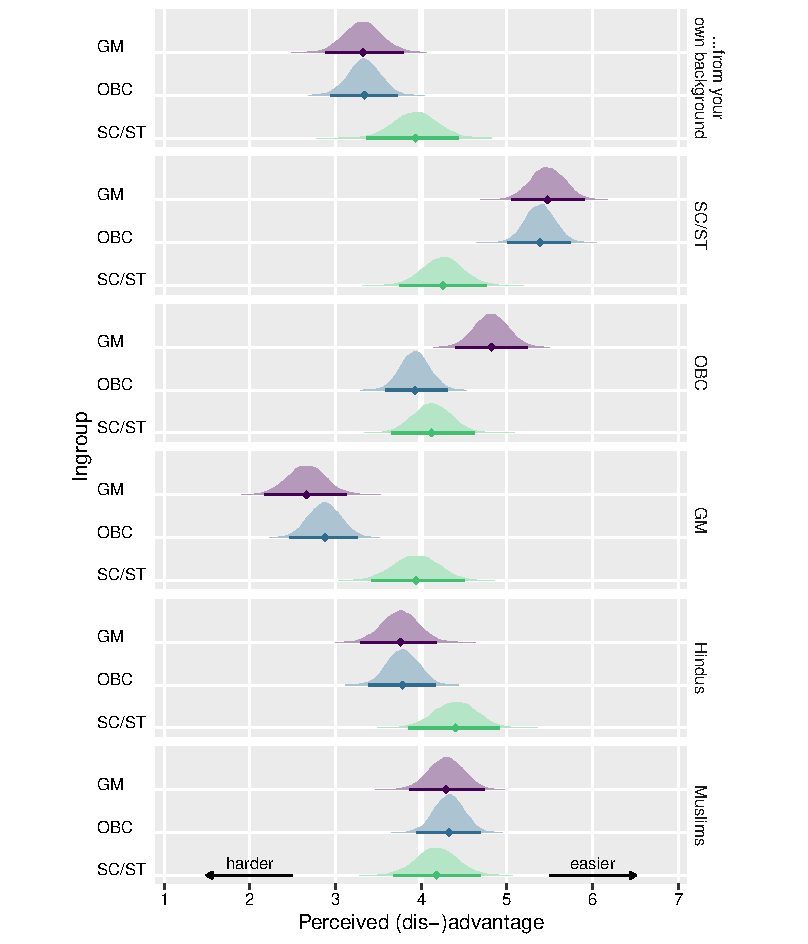
\includegraphics[scale=1]{../figures/figure-7}
\caption{
Posterior probabilities of perceived (dis-)advantage ratings for different target groups (right) by participants' caste ingroup (left). Diamonds mark the most plausible estimate of each mean rating; intervals encompass the 97\% most plausible estimates. GM = General Merit, OBC = Other Backward Class, SC/ST = Scheduled Caste/Scheduled Tribe.
}
\label{fig:f7}
\end{figure}

\begin{figure}
\centering
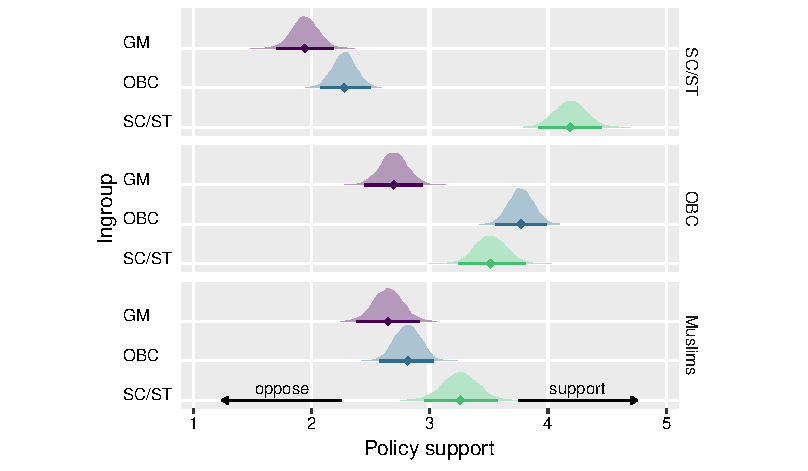
\includegraphics[scale=1]{../figures/figure-8}
\caption{
Posterior probabilities of policy support ratings for different target groups (right) by participants' caste ingroup (left). Diamonds mark the most plausible estimate of each mean rating; intervals encompass the 97\% most plausible estimates. GM = General Merit, OBC = Other Backward Class, SC/ST = Scheduled Caste/Scheduled Tribe.
}
\label{fig:f8}
\end{figure}

Overall, we found that when participants included a person in their ingroup, they had, on average, more favourable attitudes to and desired less social distance from that person. Participants' categorizations, however, were unrelated to perceptions of intergroup threat and relative (dis-)advantage, and to support for affirmative action.

\subsection{Discussion}

This research examined how people construct their social identities from multiple cross-cutting categories, and how these identities relate to intergroup contact and intergroup attitudes. As hypothesised, we found that cross-group friendship was associated with more inclusive identities which, in turn, were associated with more favourable outgroup attitudes. Negative contact was associated with less inclusive identities. Below, we discuss strengths, limitations, and implications of the research.

Our findings show that the triple crossed-categorization task \cite{dommelen_construing_2015} is an intuitive and informative method for studying social identification across multiple categories. We adapted the task to answer new questions about social identification. First, we recruited respondents from multiple groups, allowing us to study both individual and group differences (see also \citeNP{brankovic_social_2015}). Second, we estimated responses as varying across targets and participants using multilevel models. This allowed more fine-grained analyses than \citeauthor{dommelen_construing_2015}’s quantitative and qualitative summaries, and may explain why we found more consistent effects of intergroup contact. Overall, these changes open the triple crossed-categorization task to a broader range of research questions.

Still, our research is qualified by some methodological limitations. We presented all participants with the same combination of target groups. This design cannot determine whether the observed construals generalise beyond the specific combination of stimuli used. Relatedly, we did not control for factors that correlate with the categories under study, but were not made explicit. Class, rather than caste, could explain why some participants excluded targets from disadvantaged outgroups. Further, we measured categorization and attitudes for the same targets. This design cannot rule out that these variables measure the same construct, rather than represent an association across constructs. Intergroup threat, a more distal measure, did not correlate with participants' categorizations.\footnote{An explanation for this finding might be that threat perceptions stem from economic anxieties (e.g., fearing affirmative action as a threat to one's career) and ideological beliefs (e.g., Hindutva), rather than identity processes.} Future research should address these limitations by varying target categories across participants, by including more target categories, by assessing intergroup bias with proximal and distal measures, and by testing the hypothesised relationships over time.

Our research has implications for understanding intergroup relations in unequal societies. Among advantaged groups, our research documented patterns of inclusion and exclusion that map onto persistent social divides. Participants from dominant caste groups tended to exclude subordinate caste groups from the common ingroup. Hindu participants tended to exclude Indian Muslims. Among disadvantaged groups, we found more complex patterns of inclusion and exclusion. Participants from intermediate caste groups (OBC) faced the choice of aligning themselves with dominant caste groups (GM), or forming a coalition with subordinate caste groups (SC/ST). OBC participants tended to include dominant GM targets and exclude subordinate SC/ST targets, thus choosing derogation over coalition \cite{craig_coalition_2012}. Similarly, SC/ST participants rejected a solidarity-based identity that includes Indian Muslims.

Our findings suggest that cross-group friendship can overcome these divisions by fostering social identities that include Indians of all castes and religions. As more inclusive identities were related to less social distance and more warmth toward caste and religious minorities, our research suggests that positive contact could help reduce interpersonal discrimination and violence against these groups. In line with recent research (e.g., \citeNP{hayward_how_2018}), we found that negative contact could exacerbate social divisions by fostering less inclusive identities. More broadly, our research speaks to \emph{how} contact reduces prejudice \cite{pettigrew_how_2008}. Our findings support arguments \cite{gaertner_reducing_2000, pettigrew_intergroup_1998} that contact can reduce prejudice by changing how we understand our social identities.

Our research also examined support for social change. Contrary to past research, neither positive nor negative contact \cite{reimer_intergroup_2017} were associated with support for social change in advantaged \cite{dixon_intergroup_2007} and disadvantaged \cite{dixon_beyond_2012} groups. Similarly, more inclusive identities were not associated with opposition to affirmative action among the disadvantaged \cite{dovidio_darker_2012}. Features of the participants' situation might explain this discrepancy. As university students, participants have personally experienced the impact of reservation policies. For SC/ST and OBC students, reservation policies facilitated admission to state-funded universities. This experience  might explain why these students strongly support reservation (at least for their own group). For GM students, reservation policies thwarted admission to state-funded universities. This experience might explain why, in contrast to societal realities, GM students saw themselves at a disadvantage relative to other caste groups (see \citeNP{norton_whites_2011}).

To conclude, we found correlational evidence that intergroup contact can change not only how we see others, but also how we see ourselves. That is, intergroup contact can foster more inclusive social identities---and thus improve intergroup relations. Fostering more inclusive identities, however, does not seem to overcome entrenched opposition to (or undermine support for) affirmative action.

\nolinenumbers
\bibliographystyle{apacite}
\bibliography{references}

\end{document}